\section{Automatización en Scripts Bash}
Con el objetivo de agilizar el desarrollo, reducir errores manuales y estandarizar los flujos de trabajo del proyecto, se ha implementado un conjunto de automatizaciones en Bash. Estos scripts se encuentran ubicados en la carpeta \texttt{automations/} en la raíz del repositorio y automatizan tareas esenciales.

\subsection{Clonación e instalación del proyecto}
Para facilitar la integración del entorno y descargar el proyecto rápidamente, se creó el script \texttt{clone\_and\_setup.sh}. Este archivo se encarga de clonar automáticamente el repositorio desde GitHub y, secuencialmente, procede a instalar todas las dependencias necesarias. Para el Frontend utiliza \texttt{pnpm} y para el Backend utiliza el gestor de paquetes \texttt{uv}.

\begin{lstlisting}[language=bash, caption={Comando para clonar y preparar el entorno}]
./automations/clone_and_setup.sh
\end{lstlisting}

\subsection{Ejecución automatizada de los tests}
Para garantizar la integridad del código en ambas partes del sistema, se estructuró el script \texttt{run\_tests.sh}. Este unifica la ejecución de todas las pruebas automatizadas del monorepo. De forma secuencial, corre las pruebas unitarias del Frontend (usando el test runner de Node.js) y las pruebas del Backend (usando \texttt{pytest}). Si cualquiera de los dos entornos reporta fallos, el script notifica el error y devuelve un código de salida fallido, ideal para integrarse a flujos de integración continua (CI).

Un detalle de diseño: el script \emph{no} se detiene en la primera suite que falla. Guarda el código de salida de cada una y decide al final, de modo que una sola ejecución informa el estado de ambas partes del sistema en lugar de ocultar los fallos del backend detrás de un fallo del frontend.

\begin{lstlisting}[language=bash, caption={Agregación de resultados en \texttt{run\_tests.sh}}]
pnpm run test
FRONTEND_STATUS=$?
...
uv run pytest
BACKEND_STATUS=$?
...
if [ $FRONTEND_STATUS -ne 0 ] || [ $BACKEND_STATUS -ne 0 ]; then
  echo "Algunos tests han fallado."
  exit 1
fi
\end{lstlisting}

\begin{lstlisting}[language=bash, caption={Comando para ejecutar todas las pruebas}]
./automations/run_tests.sh
\end{lstlisting}

\subsection{Ejecución del proyecto en modo local}
Levantar múltiples servidores de forma separada puede ser tedioso. Para solucionar esto, se diseñó \texttt{run\_local.sh}, el cual arranca simultáneamente el servidor de desarrollo de FastAPI (puerto 8000) y el servidor de Next.js (puerto 3000) corriendo procesos en segundo plano. El script cuenta con un manejador de señales (\textit{trap}) que detecta cuando el usuario interrumpe la consola (usando \texttt{Ctrl+C}) para apagar ambos procesos de manera segura y evitar tareas remanentes.

El manejador se registra para \texttt{SIGINT}, \texttt{SIGTERM} y \texttt{EXIT} y ejecuta \texttt{kill 0}, que envía la señal a todo el grupo de procesos del script: así se detienen los dos servidores aunque el script termine por un error y no solo por \texttt{Ctrl+C}. El \texttt{wait} final mantiene el script vivo mientras los servidores corren.

\begin{lstlisting}[language=bash, caption={Manejo de señales en \texttt{run\_local.sh}}]
trap 'echo "Deteniendo servidores..."; kill 0' SIGINT SIGTERM EXIT

cd backend || exit
uv run fastapi dev main.py --port 8000 &
cd ..

cd frontend || exit
pnpm run dev &
cd ..

wait
\end{lstlisting}

\begin{lstlisting}[language=bash, caption={Comando para levantar los servidores en local}]
./automations/run_local.sh
\end{lstlisting}

\subsection{Levantamiento automatizado de contenedores Docker}
Adicional a la ejecución local, se implementó el script \texttt{run\_docker.sh} para automatizar la orquestación del proyecto mediante contenedores. El archivo invoca a Docker Compose apuntando al archivo de configuración pertinente (\texttt{docker/docker-compose.yaml}) y levanta todos los servicios en segundo plano (\textit{detached mode}).

Antes de invocar Compose, el script verifica que exista \texttt{docker/docker-compose.yaml}; si no lo encuentra, indica que debe ejecutarse desde la raíz del repositorio y termina con código de error, en lugar de fallar con un mensaje críptico de Docker. Al terminar imprime los comandos para consultar el estado, seguir los logs y detener el stack.

\begin{lstlisting}[language=bash, caption={Comando para inicializar los contenedores}]
./automations/run_docker.sh
\end{lstlisting}

\begin{figure}[H]
    \centering
    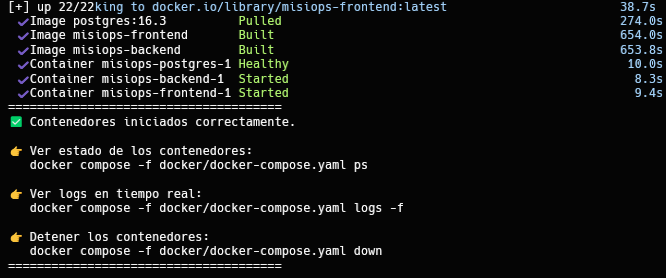
\includegraphics[width=0.85\textwidth]{figures/automation/run-docker.png}
    \caption{Ejecución de \texttt{run\_docker.sh}: construcción de imágenes y arranque de los tres contenedores, con Postgres \emph{Healthy} antes de iniciar el backend}
    \label{fig:run_docker}
\end{figure}

\subsection{Detención automatizada de contenedores Docker}
De igual manera, para asegurar que los recursos de red y contenedores se liberen de forma limpia y correcta, se creó el script \texttt{stop\_docker.sh}. Por defecto, este comando apaga y elimina los contenedores orquestados previamente por Docker Compose preservando los volúmenes de datos y las imágenes para agilizar arranques futuros. Si se desea una limpieza total (incluyendo volúmenes), el script acepta el parámetro opcional \texttt{--clean}, que añade \texttt{--volumes} a \texttt{docker compose down} y borra la base de datos para arrancar desde cero la próxima vez.

\begin{lstlisting}[language=bash, caption={Detener los contenedores preservando datos, o con limpieza total}]
./automations/stop_docker.sh           # conserva volúmenes e imágenes
./automations/stop_docker.sh --clean   # elimina también los volúmenes
\end{lstlisting}
